% Options for packages loaded elsewhere
\PassOptionsToPackage{unicode}{hyperref}
\PassOptionsToPackage{hyphens}{url}
%
\documentclass[
]{article}
\usepackage{amsmath,amssymb}
\usepackage{iftex}
\ifPDFTeX
  \usepackage[T1]{fontenc}
  \usepackage[utf8]{inputenc}
  \usepackage{textcomp} % provide euro and other symbols
\else % if luatex or xetex
  \usepackage{unicode-math} % this also loads fontspec
  \defaultfontfeatures{Scale=MatchLowercase}
  \defaultfontfeatures[\rmfamily]{Ligatures=TeX,Scale=1}
\fi
\usepackage{lmodern}
\ifPDFTeX\else
  % xetex/luatex font selection
\fi
% Use upquote if available, for straight quotes in verbatim environments
\IfFileExists{upquote.sty}{\usepackage{upquote}}{}
\IfFileExists{microtype.sty}{% use microtype if available
  \usepackage[]{microtype}
  \UseMicrotypeSet[protrusion]{basicmath} % disable protrusion for tt fonts
}{}
\makeatletter
\@ifundefined{KOMAClassName}{% if non-KOMA class
  \IfFileExists{parskip.sty}{%
    \usepackage{parskip}
  }{% else
    \setlength{\parindent}{0pt}
    \setlength{\parskip}{6pt plus 2pt minus 1pt}}
}{% if KOMA class
  \KOMAoptions{parskip=half}}
\makeatother
\usepackage{xcolor}
\usepackage[margin=1in]{geometry}
\usepackage{longtable,booktabs,array}
\usepackage{calc} % for calculating minipage widths
% Correct order of tables after \paragraph or \subparagraph
\usepackage{etoolbox}
\makeatletter
\patchcmd\longtable{\par}{\if@noskipsec\mbox{}\fi\par}{}{}
\makeatother
% Allow footnotes in longtable head/foot
\IfFileExists{footnotehyper.sty}{\usepackage{footnotehyper}}{\usepackage{footnote}}
\makesavenoteenv{longtable}
\usepackage{graphicx}
\makeatletter
\def\maxwidth{\ifdim\Gin@nat@width>\linewidth\linewidth\else\Gin@nat@width\fi}
\def\maxheight{\ifdim\Gin@nat@height>\textheight\textheight\else\Gin@nat@height\fi}
\makeatother
% Scale images if necessary, so that they will not overflow the page
% margins by default, and it is still possible to overwrite the defaults
% using explicit options in \includegraphics[width, height, ...]{}
\setkeys{Gin}{width=\maxwidth,height=\maxheight,keepaspectratio}
% Set default figure placement to htbp
\makeatletter
\def\fps@figure{htbp}
\makeatother
\setlength{\emergencystretch}{3em} % prevent overfull lines
\providecommand{\tightlist}{%
  \setlength{\itemsep}{0pt}\setlength{\parskip}{0pt}}
\setcounter{secnumdepth}{-\maxdimen} % remove section numbering
\usepackage{fontspec}
\setmainfont{NanumGothic}
\ifLuaTeX
  \usepackage{selnolig}  % disable illegal ligatures
\fi
\usepackage{bookmark}
\IfFileExists{xurl.sty}{\usepackage{xurl}}{} % add URL line breaks if available
\urlstyle{same}
\hypersetup{
  pdftitle={Literacy 250331},
  pdfauthor={coop711},
  hidelinks,
  pdfcreator={LaTeX via pandoc}}

\title{Literacy 250331}
\author{coop711}
\date{2025-03-31}

\begin{document}
\maketitle

\section{국민문해력조사 집계
결과}\label{uxad6duxbbfcuxbb38uxd574uxb825uxc870uxc0ac-uxc9d1uxacc4-uxacb0uxacfc}

\subsection{응답 집계}\label{uxc751uxb2f5-uxc9d1uxacc4}

\begin{longtable}[]{@{}
  >{\raggedleft\arraybackslash}p{(\columnwidth - 48\tabcolsep) * \real{0.0400}}
  >{\raggedleft\arraybackslash}p{(\columnwidth - 48\tabcolsep) * \real{0.0400}}
  >{\raggedleft\arraybackslash}p{(\columnwidth - 48\tabcolsep) * \real{0.0400}}
  >{\raggedleft\arraybackslash}p{(\columnwidth - 48\tabcolsep) * \real{0.0400}}
  >{\raggedleft\arraybackslash}p{(\columnwidth - 48\tabcolsep) * \real{0.0400}}
  >{\raggedleft\arraybackslash}p{(\columnwidth - 48\tabcolsep) * \real{0.0400}}
  >{\raggedleft\arraybackslash}p{(\columnwidth - 48\tabcolsep) * \real{0.0400}}
  >{\raggedleft\arraybackslash}p{(\columnwidth - 48\tabcolsep) * \real{0.0400}}
  >{\raggedleft\arraybackslash}p{(\columnwidth - 48\tabcolsep) * \real{0.0400}}
  >{\raggedleft\arraybackslash}p{(\columnwidth - 48\tabcolsep) * \real{0.0400}}
  >{\raggedleft\arraybackslash}p{(\columnwidth - 48\tabcolsep) * \real{0.0400}}
  >{\raggedleft\arraybackslash}p{(\columnwidth - 48\tabcolsep) * \real{0.0400}}
  >{\raggedleft\arraybackslash}p{(\columnwidth - 48\tabcolsep) * \real{0.0400}}
  >{\raggedleft\arraybackslash}p{(\columnwidth - 48\tabcolsep) * \real{0.0400}}
  >{\raggedleft\arraybackslash}p{(\columnwidth - 48\tabcolsep) * \real{0.0400}}
  >{\raggedleft\arraybackslash}p{(\columnwidth - 48\tabcolsep) * \real{0.0400}}
  >{\raggedleft\arraybackslash}p{(\columnwidth - 48\tabcolsep) * \real{0.0400}}
  >{\raggedleft\arraybackslash}p{(\columnwidth - 48\tabcolsep) * \real{0.0400}}
  >{\raggedleft\arraybackslash}p{(\columnwidth - 48\tabcolsep) * \real{0.0400}}
  >{\raggedleft\arraybackslash}p{(\columnwidth - 48\tabcolsep) * \real{0.0400}}
  >{\raggedleft\arraybackslash}p{(\columnwidth - 48\tabcolsep) * \real{0.0400}}
  >{\raggedleft\arraybackslash}p{(\columnwidth - 48\tabcolsep) * \real{0.0400}}
  >{\raggedleft\arraybackslash}p{(\columnwidth - 48\tabcolsep) * \real{0.0400}}
  >{\raggedleft\arraybackslash}p{(\columnwidth - 48\tabcolsep) * \real{0.0400}}
  >{\raggedleft\arraybackslash}p{(\columnwidth - 48\tabcolsep) * \real{0.0400}}@{}}
\caption{Counts}\tabularnewline
\toprule\noalign{}
\begin{minipage}[b]{\linewidth}\raggedleft
Q1
\end{minipage} & \begin{minipage}[b]{\linewidth}\raggedleft
Q2
\end{minipage} & \begin{minipage}[b]{\linewidth}\raggedleft
Q3
\end{minipage} & \begin{minipage}[b]{\linewidth}\raggedleft
Q4
\end{minipage} & \begin{minipage}[b]{\linewidth}\raggedleft
Q5
\end{minipage} & \begin{minipage}[b]{\linewidth}\raggedleft
Q6
\end{minipage} & \begin{minipage}[b]{\linewidth}\raggedleft
Q7
\end{minipage} & \begin{minipage}[b]{\linewidth}\raggedleft
Q8
\end{minipage} & \begin{minipage}[b]{\linewidth}\raggedleft
Q9
\end{minipage} & \begin{minipage}[b]{\linewidth}\raggedleft
Q10
\end{minipage} & \begin{minipage}[b]{\linewidth}\raggedleft
Q11
\end{minipage} & \begin{minipage}[b]{\linewidth}\raggedleft
Q12
\end{minipage} & \begin{minipage}[b]{\linewidth}\raggedleft
Q13
\end{minipage} & \begin{minipage}[b]{\linewidth}\raggedleft
Q14
\end{minipage} & \begin{minipage}[b]{\linewidth}\raggedleft
Q15
\end{minipage} & \begin{minipage}[b]{\linewidth}\raggedleft
Q16
\end{minipage} & \begin{minipage}[b]{\linewidth}\raggedleft
Q17
\end{minipage} & \begin{minipage}[b]{\linewidth}\raggedleft
Q18
\end{minipage} & \begin{minipage}[b]{\linewidth}\raggedleft
Q19
\end{minipage} & \begin{minipage}[b]{\linewidth}\raggedleft
Q20
\end{minipage} & \begin{minipage}[b]{\linewidth}\raggedleft
Q21
\end{minipage} & \begin{minipage}[b]{\linewidth}\raggedleft
Q22
\end{minipage} & \begin{minipage}[b]{\linewidth}\raggedleft
Q23
\end{minipage} & \begin{minipage}[b]{\linewidth}\raggedleft
Q24
\end{minipage} & \begin{minipage}[b]{\linewidth}\raggedleft
Q25
\end{minipage} \\
\midrule\noalign{}
\endfirsthead
\toprule\noalign{}
\begin{minipage}[b]{\linewidth}\raggedleft
Q1
\end{minipage} & \begin{minipage}[b]{\linewidth}\raggedleft
Q2
\end{minipage} & \begin{minipage}[b]{\linewidth}\raggedleft
Q3
\end{minipage} & \begin{minipage}[b]{\linewidth}\raggedleft
Q4
\end{minipage} & \begin{minipage}[b]{\linewidth}\raggedleft
Q5
\end{minipage} & \begin{minipage}[b]{\linewidth}\raggedleft
Q6
\end{minipage} & \begin{minipage}[b]{\linewidth}\raggedleft
Q7
\end{minipage} & \begin{minipage}[b]{\linewidth}\raggedleft
Q8
\end{minipage} & \begin{minipage}[b]{\linewidth}\raggedleft
Q9
\end{minipage} & \begin{minipage}[b]{\linewidth}\raggedleft
Q10
\end{minipage} & \begin{minipage}[b]{\linewidth}\raggedleft
Q11
\end{minipage} & \begin{minipage}[b]{\linewidth}\raggedleft
Q12
\end{minipage} & \begin{minipage}[b]{\linewidth}\raggedleft
Q13
\end{minipage} & \begin{minipage}[b]{\linewidth}\raggedleft
Q14
\end{minipage} & \begin{minipage}[b]{\linewidth}\raggedleft
Q15
\end{minipage} & \begin{minipage}[b]{\linewidth}\raggedleft
Q16
\end{minipage} & \begin{minipage}[b]{\linewidth}\raggedleft
Q17
\end{minipage} & \begin{minipage}[b]{\linewidth}\raggedleft
Q18
\end{minipage} & \begin{minipage}[b]{\linewidth}\raggedleft
Q19
\end{minipage} & \begin{minipage}[b]{\linewidth}\raggedleft
Q20
\end{minipage} & \begin{minipage}[b]{\linewidth}\raggedleft
Q21
\end{minipage} & \begin{minipage}[b]{\linewidth}\raggedleft
Q22
\end{minipage} & \begin{minipage}[b]{\linewidth}\raggedleft
Q23
\end{minipage} & \begin{minipage}[b]{\linewidth}\raggedleft
Q24
\end{minipage} & \begin{minipage}[b]{\linewidth}\raggedleft
Q25
\end{minipage} \\
\midrule\noalign{}
\endhead
\bottomrule\noalign{}
\endlastfoot
0 & 5 & 420 & 7 & 6 & 43 & 502 & 37 & 47 & 8 & 480 & 17 & 10 & 18 & 22 &
443 & 137 & 11 & 495 & 34 & 25 & 33 & 487 & 56 & 15 \\
8 & 3 & 31 & 8 & 482 & 38 & 17 & 35 & 297 & 483 & 24 & 153 & 474 & 30 &
59 & 44 & 33 & 492 & 16 & 52 & 440 & 68 & 26 & 28 & 441 \\
537 & 27 & 19 & 521 & 44 & 90 & 17 & 39 & 186 & 31 & 27 & 362 & 30 & 21
& 395 & 37 & 21 & 37 & 20 & 441 & 31 & 45 & 17 & 435 & 69 \\
1 & 511 & 76 & 10 & 14 & 375 & 10 & 435 & 16 & 24 & 15 & 14 & 32 & 477 &
70 & 22 & 355 & 6 & 15 & 19 & 50 & 400 & 16 & 27 & 21 \\
\end{longtable}

\begin{longtable}[]{@{}
  >{\raggedleft\arraybackslash}p{(\columnwidth - 48\tabcolsep) * \real{0.0330}}
  >{\raggedleft\arraybackslash}p{(\columnwidth - 48\tabcolsep) * \real{0.0330}}
  >{\raggedleft\arraybackslash}p{(\columnwidth - 48\tabcolsep) * \real{0.0330}}
  >{\raggedleft\arraybackslash}p{(\columnwidth - 48\tabcolsep) * \real{0.0330}}
  >{\raggedleft\arraybackslash}p{(\columnwidth - 48\tabcolsep) * \real{0.0330}}
  >{\raggedleft\arraybackslash}p{(\columnwidth - 48\tabcolsep) * \real{0.0330}}
  >{\raggedleft\arraybackslash}p{(\columnwidth - 48\tabcolsep) * \real{0.0330}}
  >{\raggedleft\arraybackslash}p{(\columnwidth - 48\tabcolsep) * \real{0.0330}}
  >{\raggedleft\arraybackslash}p{(\columnwidth - 48\tabcolsep) * \real{0.0330}}
  >{\raggedleft\arraybackslash}p{(\columnwidth - 48\tabcolsep) * \real{0.0440}}
  >{\raggedleft\arraybackslash}p{(\columnwidth - 48\tabcolsep) * \real{0.0440}}
  >{\raggedleft\arraybackslash}p{(\columnwidth - 48\tabcolsep) * \real{0.0440}}
  >{\raggedleft\arraybackslash}p{(\columnwidth - 48\tabcolsep) * \real{0.0440}}
  >{\raggedleft\arraybackslash}p{(\columnwidth - 48\tabcolsep) * \real{0.0440}}
  >{\raggedleft\arraybackslash}p{(\columnwidth - 48\tabcolsep) * \real{0.0440}}
  >{\raggedleft\arraybackslash}p{(\columnwidth - 48\tabcolsep) * \real{0.0440}}
  >{\raggedleft\arraybackslash}p{(\columnwidth - 48\tabcolsep) * \real{0.0440}}
  >{\raggedleft\arraybackslash}p{(\columnwidth - 48\tabcolsep) * \real{0.0440}}
  >{\raggedleft\arraybackslash}p{(\columnwidth - 48\tabcolsep) * \real{0.0440}}
  >{\raggedleft\arraybackslash}p{(\columnwidth - 48\tabcolsep) * \real{0.0440}}
  >{\raggedleft\arraybackslash}p{(\columnwidth - 48\tabcolsep) * \real{0.0440}}
  >{\raggedleft\arraybackslash}p{(\columnwidth - 48\tabcolsep) * \real{0.0440}}
  >{\raggedleft\arraybackslash}p{(\columnwidth - 48\tabcolsep) * \real{0.0440}}
  >{\raggedleft\arraybackslash}p{(\columnwidth - 48\tabcolsep) * \real{0.0440}}
  >{\raggedleft\arraybackslash}p{(\columnwidth - 48\tabcolsep) * \real{0.0440}}@{}}
\caption{\%}\tabularnewline
\toprule\noalign{}
\begin{minipage}[b]{\linewidth}\raggedleft
Q1
\end{minipage} & \begin{minipage}[b]{\linewidth}\raggedleft
Q2
\end{minipage} & \begin{minipage}[b]{\linewidth}\raggedleft
Q3
\end{minipage} & \begin{minipage}[b]{\linewidth}\raggedleft
Q4
\end{minipage} & \begin{minipage}[b]{\linewidth}\raggedleft
Q5
\end{minipage} & \begin{minipage}[b]{\linewidth}\raggedleft
Q6
\end{minipage} & \begin{minipage}[b]{\linewidth}\raggedleft
Q7
\end{minipage} & \begin{minipage}[b]{\linewidth}\raggedleft
Q8
\end{minipage} & \begin{minipage}[b]{\linewidth}\raggedleft
Q9
\end{minipage} & \begin{minipage}[b]{\linewidth}\raggedleft
Q10
\end{minipage} & \begin{minipage}[b]{\linewidth}\raggedleft
Q11
\end{minipage} & \begin{minipage}[b]{\linewidth}\raggedleft
Q12
\end{minipage} & \begin{minipage}[b]{\linewidth}\raggedleft
Q13
\end{minipage} & \begin{minipage}[b]{\linewidth}\raggedleft
Q14
\end{minipage} & \begin{minipage}[b]{\linewidth}\raggedleft
Q15
\end{minipage} & \begin{minipage}[b]{\linewidth}\raggedleft
Q16
\end{minipage} & \begin{minipage}[b]{\linewidth}\raggedleft
Q17
\end{minipage} & \begin{minipage}[b]{\linewidth}\raggedleft
Q18
\end{minipage} & \begin{minipage}[b]{\linewidth}\raggedleft
Q19
\end{minipage} & \begin{minipage}[b]{\linewidth}\raggedleft
Q20
\end{minipage} & \begin{minipage}[b]{\linewidth}\raggedleft
Q21
\end{minipage} & \begin{minipage}[b]{\linewidth}\raggedleft
Q22
\end{minipage} & \begin{minipage}[b]{\linewidth}\raggedleft
Q23
\end{minipage} & \begin{minipage}[b]{\linewidth}\raggedleft
Q24
\end{minipage} & \begin{minipage}[b]{\linewidth}\raggedleft
Q25
\end{minipage} \\
\midrule\noalign{}
\endfirsthead
\toprule\noalign{}
\begin{minipage}[b]{\linewidth}\raggedleft
Q1
\end{minipage} & \begin{minipage}[b]{\linewidth}\raggedleft
Q2
\end{minipage} & \begin{minipage}[b]{\linewidth}\raggedleft
Q3
\end{minipage} & \begin{minipage}[b]{\linewidth}\raggedleft
Q4
\end{minipage} & \begin{minipage}[b]{\linewidth}\raggedleft
Q5
\end{minipage} & \begin{minipage}[b]{\linewidth}\raggedleft
Q6
\end{minipage} & \begin{minipage}[b]{\linewidth}\raggedleft
Q7
\end{minipage} & \begin{minipage}[b]{\linewidth}\raggedleft
Q8
\end{minipage} & \begin{minipage}[b]{\linewidth}\raggedleft
Q9
\end{minipage} & \begin{minipage}[b]{\linewidth}\raggedleft
Q10
\end{minipage} & \begin{minipage}[b]{\linewidth}\raggedleft
Q11
\end{minipage} & \begin{minipage}[b]{\linewidth}\raggedleft
Q12
\end{minipage} & \begin{minipage}[b]{\linewidth}\raggedleft
Q13
\end{minipage} & \begin{minipage}[b]{\linewidth}\raggedleft
Q14
\end{minipage} & \begin{minipage}[b]{\linewidth}\raggedleft
Q15
\end{minipage} & \begin{minipage}[b]{\linewidth}\raggedleft
Q16
\end{minipage} & \begin{minipage}[b]{\linewidth}\raggedleft
Q17
\end{minipage} & \begin{minipage}[b]{\linewidth}\raggedleft
Q18
\end{minipage} & \begin{minipage}[b]{\linewidth}\raggedleft
Q19
\end{minipage} & \begin{minipage}[b]{\linewidth}\raggedleft
Q20
\end{minipage} & \begin{minipage}[b]{\linewidth}\raggedleft
Q21
\end{minipage} & \begin{minipage}[b]{\linewidth}\raggedleft
Q22
\end{minipage} & \begin{minipage}[b]{\linewidth}\raggedleft
Q23
\end{minipage} & \begin{minipage}[b]{\linewidth}\raggedleft
Q24
\end{minipage} & \begin{minipage}[b]{\linewidth}\raggedleft
Q25
\end{minipage} \\
\midrule\noalign{}
\endhead
\bottomrule\noalign{}
\endlastfoot
0 & 1 & 77 & 1 & 1 & 8 & 92 & 7 & 9 & 1 & 88 & 3 & 2 & 3 & 4 & 81 & 25 &
2 & 91 & 6 & 5 & 6 & 89 & 10 & 3 \\
1 & 1 & 6 & 1 & 88 & 7 & 3 & 6 & 54 & 88 & 4 & 28 & 87 & 5 & 11 & 8 & 6
& 90 & 3 & 10 & 81 & 12 & 5 & 5 & 81 \\
98 & 5 & 3 & 95 & 8 & 16 & 3 & 7 & 34 & 6 & 5 & 66 & 5 & 4 & 72 & 7 & 4
& 7 & 4 & 81 & 6 & 8 & 3 & 80 & 13 \\
0 & 94 & 14 & 2 & 3 & 69 & 2 & 80 & 3 & 4 & 3 & 3 & 6 & 87 & 13 & 4 & 65
& 1 & 3 & 3 & 9 & 73 & 3 & 5 & 4 \\
\end{longtable}

\subsection{막대그래프}\label{uxb9c9uxb300uxadf8uxb798uxd504}

막대그래프로 답안 분포를 시각적으로 살핀다. 차후 나오는 정답률과 함께
어느 문항에서 어느 답안을 많이 고르는지 파악하는 데 활용한다.

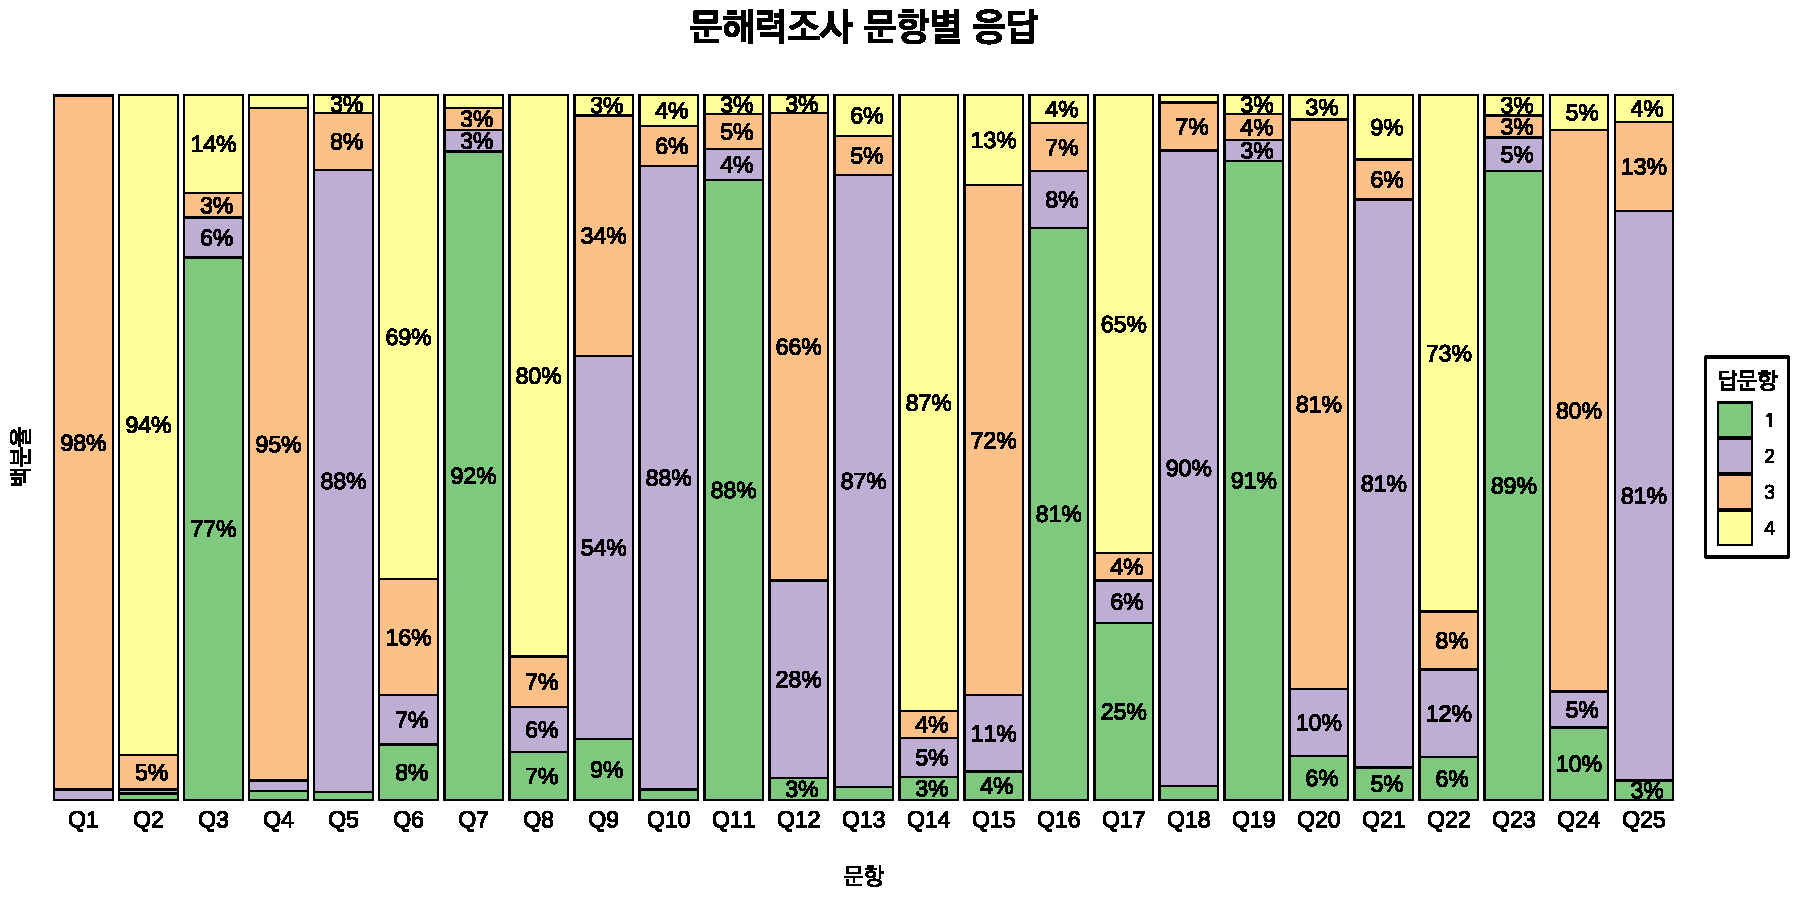
\includegraphics{Literacy_google_p_250331_v3_files/figure-latex/unnamed-chunk-5-1.pdf}

\subsection{문해력 점수
계산}\label{uxbb38uxd574uxb825-uxc810uxc218-uxacc4uxc0b0}

\subsubsection{정답과 대조하여 R(Right)/W(Wrong)
표시}\label{uxc815uxb2f5uxacfc-uxb300uxc870uxd558uxc5ec-rrightwwrong-uxd45cuxc2dc}

\begin{longtable}[]{@{}
  >{\raggedleft\arraybackslash}p{(\columnwidth - 48\tabcolsep) * \real{0.0355}}
  >{\raggedleft\arraybackslash}p{(\columnwidth - 48\tabcolsep) * \real{0.0355}}
  >{\raggedleft\arraybackslash}p{(\columnwidth - 48\tabcolsep) * \real{0.0355}}
  >{\raggedleft\arraybackslash}p{(\columnwidth - 48\tabcolsep) * \real{0.0355}}
  >{\raggedleft\arraybackslash}p{(\columnwidth - 48\tabcolsep) * \real{0.0355}}
  >{\raggedleft\arraybackslash}p{(\columnwidth - 48\tabcolsep) * \real{0.0355}}
  >{\raggedleft\arraybackslash}p{(\columnwidth - 48\tabcolsep) * \real{0.0355}}
  >{\raggedleft\arraybackslash}p{(\columnwidth - 48\tabcolsep) * \real{0.0355}}
  >{\raggedleft\arraybackslash}p{(\columnwidth - 48\tabcolsep) * \real{0.0355}}
  >{\raggedleft\arraybackslash}p{(\columnwidth - 48\tabcolsep) * \real{0.0426}}
  >{\raggedleft\arraybackslash}p{(\columnwidth - 48\tabcolsep) * \real{0.0426}}
  >{\raggedleft\arraybackslash}p{(\columnwidth - 48\tabcolsep) * \real{0.0426}}
  >{\raggedleft\arraybackslash}p{(\columnwidth - 48\tabcolsep) * \real{0.0426}}
  >{\raggedleft\arraybackslash}p{(\columnwidth - 48\tabcolsep) * \real{0.0426}}
  >{\raggedleft\arraybackslash}p{(\columnwidth - 48\tabcolsep) * \real{0.0426}}
  >{\raggedleft\arraybackslash}p{(\columnwidth - 48\tabcolsep) * \real{0.0426}}
  >{\raggedleft\arraybackslash}p{(\columnwidth - 48\tabcolsep) * \real{0.0426}}
  >{\raggedleft\arraybackslash}p{(\columnwidth - 48\tabcolsep) * \real{0.0426}}
  >{\raggedleft\arraybackslash}p{(\columnwidth - 48\tabcolsep) * \real{0.0426}}
  >{\raggedleft\arraybackslash}p{(\columnwidth - 48\tabcolsep) * \real{0.0426}}
  >{\raggedleft\arraybackslash}p{(\columnwidth - 48\tabcolsep) * \real{0.0426}}
  >{\raggedleft\arraybackslash}p{(\columnwidth - 48\tabcolsep) * \real{0.0426}}
  >{\raggedleft\arraybackslash}p{(\columnwidth - 48\tabcolsep) * \real{0.0426}}
  >{\raggedleft\arraybackslash}p{(\columnwidth - 48\tabcolsep) * \real{0.0426}}
  >{\raggedleft\arraybackslash}p{(\columnwidth - 48\tabcolsep) * \real{0.0426}}@{}}
\toprule\noalign{}
\begin{minipage}[b]{\linewidth}\raggedleft
Q1
\end{minipage} & \begin{minipage}[b]{\linewidth}\raggedleft
Q2
\end{minipage} & \begin{minipage}[b]{\linewidth}\raggedleft
Q3
\end{minipage} & \begin{minipage}[b]{\linewidth}\raggedleft
Q4
\end{minipage} & \begin{minipage}[b]{\linewidth}\raggedleft
Q5
\end{minipage} & \begin{minipage}[b]{\linewidth}\raggedleft
Q6
\end{minipage} & \begin{minipage}[b]{\linewidth}\raggedleft
Q7
\end{minipage} & \begin{minipage}[b]{\linewidth}\raggedleft
Q8
\end{minipage} & \begin{minipage}[b]{\linewidth}\raggedleft
Q9
\end{minipage} & \begin{minipage}[b]{\linewidth}\raggedleft
Q10
\end{minipage} & \begin{minipage}[b]{\linewidth}\raggedleft
Q11
\end{minipage} & \begin{minipage}[b]{\linewidth}\raggedleft
Q12
\end{minipage} & \begin{minipage}[b]{\linewidth}\raggedleft
Q13
\end{minipage} & \begin{minipage}[b]{\linewidth}\raggedleft
Q14
\end{minipage} & \begin{minipage}[b]{\linewidth}\raggedleft
Q15
\end{minipage} & \begin{minipage}[b]{\linewidth}\raggedleft
Q16
\end{minipage} & \begin{minipage}[b]{\linewidth}\raggedleft
Q17
\end{minipage} & \begin{minipage}[b]{\linewidth}\raggedleft
Q18
\end{minipage} & \begin{minipage}[b]{\linewidth}\raggedleft
Q19
\end{minipage} & \begin{minipage}[b]{\linewidth}\raggedleft
Q20
\end{minipage} & \begin{minipage}[b]{\linewidth}\raggedleft
Q21
\end{minipage} & \begin{minipage}[b]{\linewidth}\raggedleft
Q22
\end{minipage} & \begin{minipage}[b]{\linewidth}\raggedleft
Q23
\end{minipage} & \begin{minipage}[b]{\linewidth}\raggedleft
Q24
\end{minipage} & \begin{minipage}[b]{\linewidth}\raggedleft
Q25
\end{minipage} \\
\midrule\noalign{}
\endhead
\bottomrule\noalign{}
\endlastfoot
R & R & R & R & R & W & W & W & W & W & R & R & R & R & R & R & R & R &
R & R & R & R & R & R & R \\
R & R & R & R & R & R & R & R & R & R & R & R & R & R & R & R & W & R &
R & R & R & R & R & R & R \\
R & R & R & R & R & R & R & R & R & R & R & R & R & R & R & R & W & R &
R & R & R & R & R & R & R \\
R & R & R & R & R & R & R & R & R & R & R & R & R & R & R & R & R & R &
R & R & R & R & R & R & R \\
R & R & R & R & R & R & R & W & W & R & R & W & R & R & W & R & W & R &
R & W & R & R & R & R & R \\
R & R & R & R & R & R & R & R & R & R & R & R & R & R & R & R & R & R &
R & R & R & R & R & R & R \\
\end{longtable}

\subsubsection{학생별 점수
산출}\label{uxd559uxc0dduxbcc4-uxc810uxc218-uxc0b0uxcd9c}

\emph{80}, \emph{96}, \emph{96}, \emph{100}, \emph{76}, \emph{100},
\emph{88}, \emph{20}, \emph{92}, \emph{92}, \emph{88}, \emph{80},
\emph{100}, \emph{100}, \emph{80}, \emph{100}, \emph{92}, \emph{84},
\emph{100}, \emph{92}, \emph{84}, \emph{100}, \emph{92}, \emph{100},
\emph{96}, \emph{92}, \emph{84}, \emph{88}, \emph{48}, \emph{92},
\emph{96}, \emph{100}, \emph{80}, \emph{96}, \emph{92}, \emph{84},
\emph{92}, \emph{72}, \emph{96}, \emph{96}, \emph{96}, \emph{60},
\emph{100}, \emph{76}, \emph{76}, \emph{72}, \emph{80}, \emph{32},
\emph{64}, \emph{88}, \emph{92}, \emph{92}, \emph{92}, \emph{88},
\emph{96}, \emph{96}, \emph{48}, \emph{84}, \emph{72}, \emph{100},
\emph{88}, \emph{88}, \emph{88}, \emph{92}, \emph{76}, \emph{96},
\emph{96}, \emph{84}, \emph{92}, \emph{88}, \emph{96}, \emph{88},
\emph{100}, \emph{68}, \emph{80}, \emph{76}, \emph{84}, \emph{92},
\emph{92}, \emph{92}, \emph{80}, \emph{88}, \emph{84}, \emph{56},
\emph{72}, \emph{80}, \emph{84}, \emph{28}, \emph{100}, \emph{96},
\emph{92}, \emph{92}, \emph{88}, \emph{84}, \emph{88}, \emph{96},
\emph{84}, \emph{84}, \emph{88}, \emph{88}, \emph{92}, \emph{88},
\emph{88}, \emph{84}, \emph{76}, \emph{88}, \emph{88}, \emph{92},
\emph{44}, \emph{80}, \emph{84}, \emph{20}, \emph{80}, \emph{72},
\emph{92}, \emph{100}, \emph{96}, \emph{92}, \emph{88}, \emph{72},
\emph{88}, \emph{64}, \emph{56}, \emph{96}, \emph{80}, \emph{92},
\emph{84}, \emph{88}, \emph{76}, \emph{80}, \emph{84}, \emph{76},
\emph{88}, \emph{36}, \emph{80}, \emph{92}, \emph{84}, \emph{68},
\emph{80}, \emph{76}, \emph{80}, \emph{96}, \emph{96}, \emph{84},
\emph{96}, \emph{88}, \emph{68}, \emph{92}, \emph{92}, \emph{88},
\emph{92}, \emph{28}, \emph{80}, \emph{44}, \emph{100}, \emph{84},
\emph{84}, \emph{96}, \emph{68}, \emph{100}, \emph{88}, \emph{84},
\emph{92}, \emph{92}, \emph{100}, \emph{96}, \emph{92}, \emph{96},
\emph{12}, \emph{92}, \emph{72}, \emph{92}, \emph{88}, \emph{100},
\emph{20}, \emph{80}, \emph{92}, \emph{100}, \emph{100}, \emph{100},
\emph{92}, \emph{100}, \emph{92}, \emph{92}, \emph{80}, \emph{84},
\emph{92}, \emph{88}, \emph{88}, \emph{100}, \emph{88}, \emph{88},
\emph{96}, \emph{92}, \emph{80}, \emph{100}, \emph{92}, \emph{88},
\emph{96}, \emph{84}, \emph{96}, \emph{96}, \emph{96}, \emph{80},
\emph{96}, \emph{96}, \emph{52}, \emph{80}, \emph{84}, \emph{68},
\emph{92}, \emph{84}, \emph{80}, \emph{48}, \emph{84}, \emph{80},
\emph{88}, \emph{84}, \emph{96}, \emph{36}, \emph{88}, \emph{92},
\emph{88}, \emph{88}, \emph{60}, \emph{80}, \emph{84}, \emph{88},
\emph{92}, \emph{84}, \emph{64}, \emph{92}, \emph{92}, \emph{96},
\emph{88}, \emph{88}, \emph{88}, \emph{88}, \emph{88}, \emph{36},
\emph{64}, \emph{84}, \emph{76}, \emph{80}, \emph{80}, \emph{24},
\emph{100}, \emph{88}, \emph{80}, \emph{88}, \emph{92}, \emph{64},
\emph{76}, \emph{80}, \emph{24}, \emph{80}, \emph{96}, \emph{56},
\emph{64}, \emph{84}, \emph{88}, \emph{64}, \emph{84}, \emph{84},
\emph{96}, \emph{84}, \emph{92}, \emph{88}, \emph{80}, \emph{84},
\emph{24}, \emph{76}, \emph{48}, \emph{96}, \emph{88}, \emph{40},
\emph{80}, \emph{84}, \emph{80}, \emph{88}, \emph{92}, \emph{92},
\emph{80}, \emph{96}, \emph{64}, \emph{96}, \emph{40}, \emph{92},
\emph{92}, \emph{88}, \emph{84}, \emph{100}, \emph{36}, \emph{80},
\emph{92}, \emph{84}, \emph{84}, \emph{32}, \emph{96}, \emph{96},
\emph{96}, \emph{96}, \emph{96}, \emph{92}, \emph{92}, \emph{96},
\emph{84}, \emph{88}, \emph{92}, \emph{92}, \emph{88}, \emph{84},
\emph{80}, \emph{100}, \emph{80}, \emph{64}, \emph{28}, \emph{92},
\emph{88}, \emph{80}, \emph{92}, \emph{100}, \emph{92}, \emph{88},
\emph{100}, \emph{84}, \emph{80}, \emph{56}, \emph{84}, \emph{16},
\emph{76}, \emph{96}, \emph{80}, \emph{84}, \emph{68}, \emph{92},
\emph{88}, \emph{84}, \emph{88}, \emph{96}, \emph{88}, \emph{56},
\emph{36}, \emph{88}, \emph{88}, \emph{72}, \emph{76}, \emph{92},
\emph{96}, \emph{80}, \emph{92}, \emph{100}, \emph{80}, \emph{48},
\emph{28}, \emph{36}, \emph{92}, \emph{88}, \emph{84}, \emph{68},
\emph{88}, \emph{36}, \emph{92}, \emph{88}, \emph{92}, \emph{72},
\emph{84}, \emph{96}, \emph{60}, \emph{88}, \emph{96}, \emph{84},
\emph{92}, \emph{72}, \emph{100}, \emph{84}, \emph{88}, \emph{96},
\emph{80}, \emph{96}, \emph{72}, \emph{96}, \emph{80}, \emph{24},
\emph{88}, \emph{96}, \emph{36}, \emph{64}, \emph{80}, \emph{88},
\emph{92}, \emph{92}, \emph{80}, \emph{96}, \emph{92}, \emph{88},
\emph{80}, \emph{96}, \emph{88}, \emph{80}, \emph{52}, \emph{92},
\emph{92}, \emph{44}, \emph{96}, \emph{44}, \emph{88}, \emph{100},
\emph{88}, \emph{92}, \emph{96}, \emph{100}, \emph{92}, \emph{96},
\emph{88}, \emph{92}, \emph{96}, \emph{36}, \emph{92}, \emph{84},
\emph{88}, \emph{92}, \emph{56}, \emph{84}, \emph{72}, \emph{84},
\emph{88}, \emph{96}, \emph{100}, \emph{96}, \emph{76}, \emph{76},
\emph{88}, \emph{88}, \emph{88}, \emph{96}, \emph{92}, \emph{28},
\emph{96}, \emph{92}, \emph{88}, \emph{84}, \emph{76}, \emph{100},
\emph{92}, \emph{92}, \emph{88}, \emph{100}, \emph{84}, \emph{60},
\emph{84}, \emph{84}, \emph{84}, \emph{76}, \emph{100}, \emph{100},
\emph{92}, \emph{16}, \emph{84}, \emph{52}, \emph{84}, \emph{88},
\emph{88}, \emph{96}, \emph{96}, \emph{88}, \emph{88}, \emph{80},
\emph{56}, \emph{92}, \emph{28}, \emph{76}, \emph{72}, \emph{96},
\emph{80}, \emph{84}, \emph{40}, \emph{88}, \emph{88}, \emph{80},
\emph{96}, \emph{76}, \emph{96}, \emph{100}, \emph{32}, \emph{76},
\emph{88}, \emph{100}, \emph{100}, \emph{36}, \emph{92}, \emph{16},
\emph{84}, \emph{96}, \emph{92}, \emph{88}, \emph{52}, \emph{80},
\emph{84}, \emph{92}, \emph{40}, \emph{96}, \emph{96}, \emph{32},
\emph{48}, \emph{60}, \emph{92}, \emph{96}, \emph{68}, \emph{48},
\emph{48}, \emph{88}, \emph{52}, \emph{92}, \emph{52}, \emph{88},
\emph{80}, \emph{24}, \emph{76}, \emph{100}, \emph{88}, \emph{92},
\emph{80}, \emph{92}, \emph{88}, \emph{20}, \emph{92}, \emph{84},
\emph{52}, \emph{96}, \emph{96}, \emph{88}, \emph{52}, \emph{84},
\emph{40}, \emph{88}, \emph{48}, \emph{60}, \emph{72}, \emph{48},
\emph{64}, \emph{60}, \emph{40}, \emph{92}, \emph{76} and \emph{28}

\subsection{Red and Black 비교}\label{red-and-black-uxbe44uxad50}

\subsubsection{Summary}\label{summary}

\begin{itemize}
\item
  \textbf{Red}:

  \begin{longtable}[]{@{}
    >{\raggedleft\arraybackslash}p{(\columnwidth - 10\tabcolsep) * \real{0.0972}}
    >{\raggedleft\arraybackslash}p{(\columnwidth - 10\tabcolsep) * \real{0.1389}}
    >{\raggedleft\arraybackslash}p{(\columnwidth - 10\tabcolsep) * \real{0.1250}}
    >{\raggedleft\arraybackslash}p{(\columnwidth - 10\tabcolsep) * \real{0.0972}}
    >{\raggedleft\arraybackslash}p{(\columnwidth - 10\tabcolsep) * \real{0.1389}}
    >{\raggedleft\arraybackslash}p{(\columnwidth - 10\tabcolsep) * \real{0.0972}}@{}}
  \toprule\noalign{}
  \begin{minipage}[b]{\linewidth}\raggedleft
  Min.
  \end{minipage} & \begin{minipage}[b]{\linewidth}\raggedleft
  1st Qu.
  \end{minipage} & \begin{minipage}[b]{\linewidth}\raggedleft
  Median
  \end{minipage} & \begin{minipage}[b]{\linewidth}\raggedleft
  Mean
  \end{minipage} & \begin{minipage}[b]{\linewidth}\raggedleft
  3rd Qu.
  \end{minipage} & \begin{minipage}[b]{\linewidth}\raggedleft
  Max.
  \end{minipage} \\
  \midrule\noalign{}
  \endhead
  \bottomrule\noalign{}
  \endlastfoot
  16 & 77 & 88 & 79.9 & 92 & 100 \\
  \end{longtable}
\item
  \textbf{Black}:

  \begin{longtable}[]{@{}
    >{\raggedleft\arraybackslash}p{(\columnwidth - 10\tabcolsep) * \real{0.0972}}
    >{\raggedleft\arraybackslash}p{(\columnwidth - 10\tabcolsep) * \real{0.1389}}
    >{\raggedleft\arraybackslash}p{(\columnwidth - 10\tabcolsep) * \real{0.1250}}
    >{\raggedleft\arraybackslash}p{(\columnwidth - 10\tabcolsep) * \real{0.0972}}
    >{\raggedleft\arraybackslash}p{(\columnwidth - 10\tabcolsep) * \real{0.1389}}
    >{\raggedleft\arraybackslash}p{(\columnwidth - 10\tabcolsep) * \real{0.0972}}@{}}
  \toprule\noalign{}
  \begin{minipage}[b]{\linewidth}\raggedleft
  Min.
  \end{minipage} & \begin{minipage}[b]{\linewidth}\raggedleft
  1st Qu.
  \end{minipage} & \begin{minipage}[b]{\linewidth}\raggedleft
  Median
  \end{minipage} & \begin{minipage}[b]{\linewidth}\raggedleft
  Mean
  \end{minipage} & \begin{minipage}[b]{\linewidth}\raggedleft
  3rd Qu.
  \end{minipage} & \begin{minipage}[b]{\linewidth}\raggedleft
  Max.
  \end{minipage} \\
  \midrule\noalign{}
  \endhead
  \bottomrule\noalign{}
  \endlastfoot
  12 & 80 & 88 & 82.2 & 92 & 100 \\
  \end{longtable}
\end{itemize}

\subsubsection{줄기-잎 그림}\label{uxc904uxae30-uxc78e-uxadf8uxb9bc}

\begin{itemize}
\tightlist
\item
  Red
\end{itemize}

\begin{verbatim}
## 
##   The decimal point is 1 digit(s) to the right of the |
## 
##    1 | 6
##    2 | 000048888
##    3 | 222666666
##    4 | 00004488888888
##    5 | 2226666
##    6 | 0000444448888
##    7 | 222266666666666
##    8 | 00000000000000000000000000000000000044444444444444444444444448888888+28
##    9 | 22222222222222222222222222222222222222666666666666666666666666666666
##   10 | 00000000000000000000
\end{verbatim}

\begin{itemize}
\tightlist
\item
  Black
\end{itemize}

\begin{verbatim}
## 
##   The decimal point is 1 digit(s) to the right of the |
## 
##    1 | 266
##    2 | 4444888
##    3 | 26666
##    4 | 004488
##    5 | 22222666
##    6 | 0004444448888
##    7 | 2222222222666666666666
##    8 | 00000000000000000444444444444444444444444444444444444444888888888888+20
##    9 | 22222222222222222222222222222222222222222222222222222666666666666666+10
##   10 | 0000000000000000000000
\end{verbatim}

\subsubsection{Box Plots}\label{box-plots}

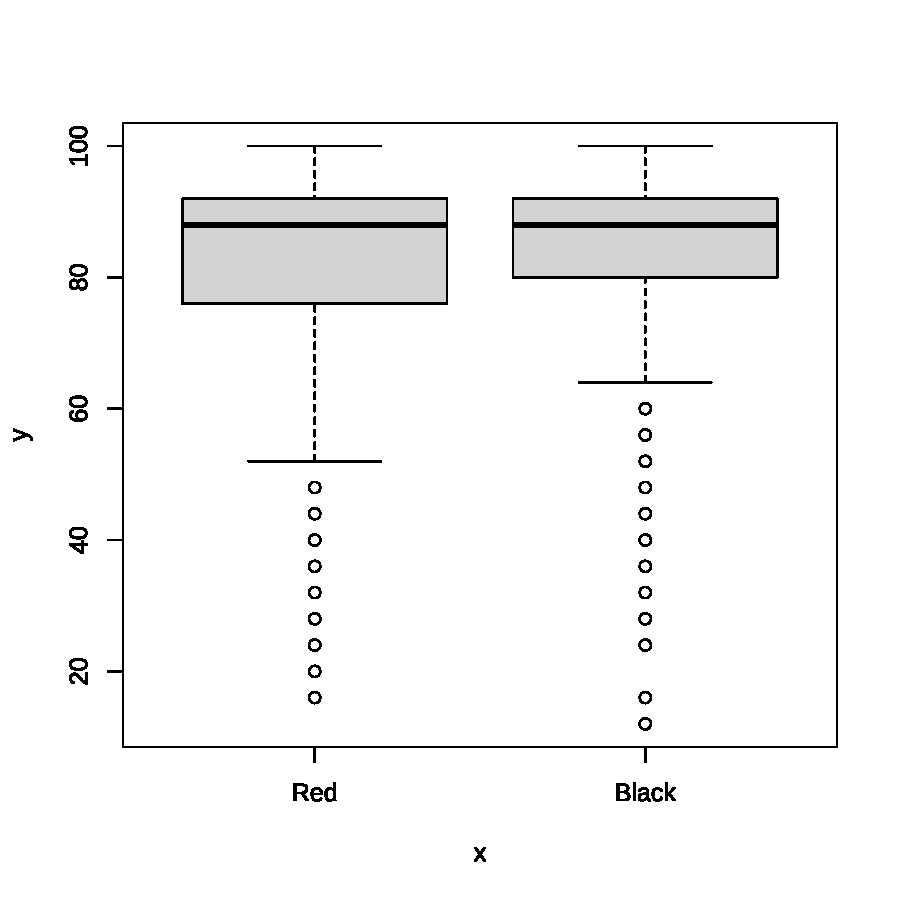
\includegraphics{Literacy_google_p_250331_v3_files/figure-latex/boxplots-1.pdf}

\subsubsection{QQ plot}\label{qq-plot}

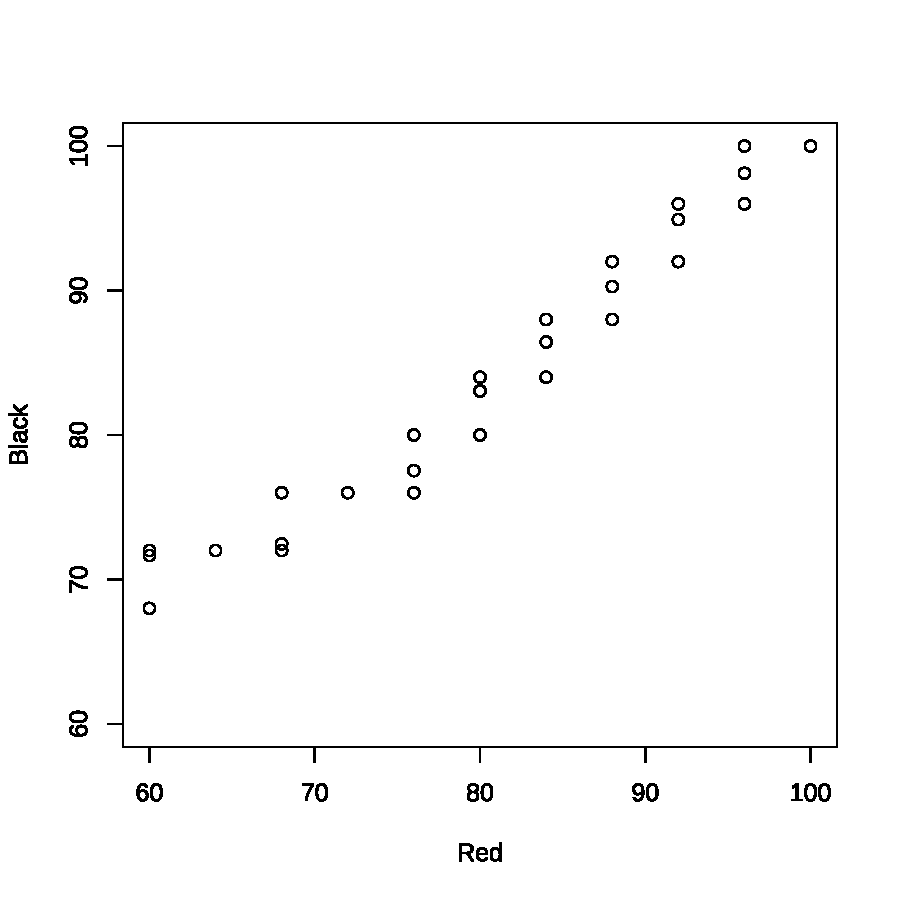
\includegraphics{Literacy_google_p_250331_v3_files/figure-latex/qqplots-1.pdf}

\subsubsection{ECDF plot}\label{ecdf-plot}

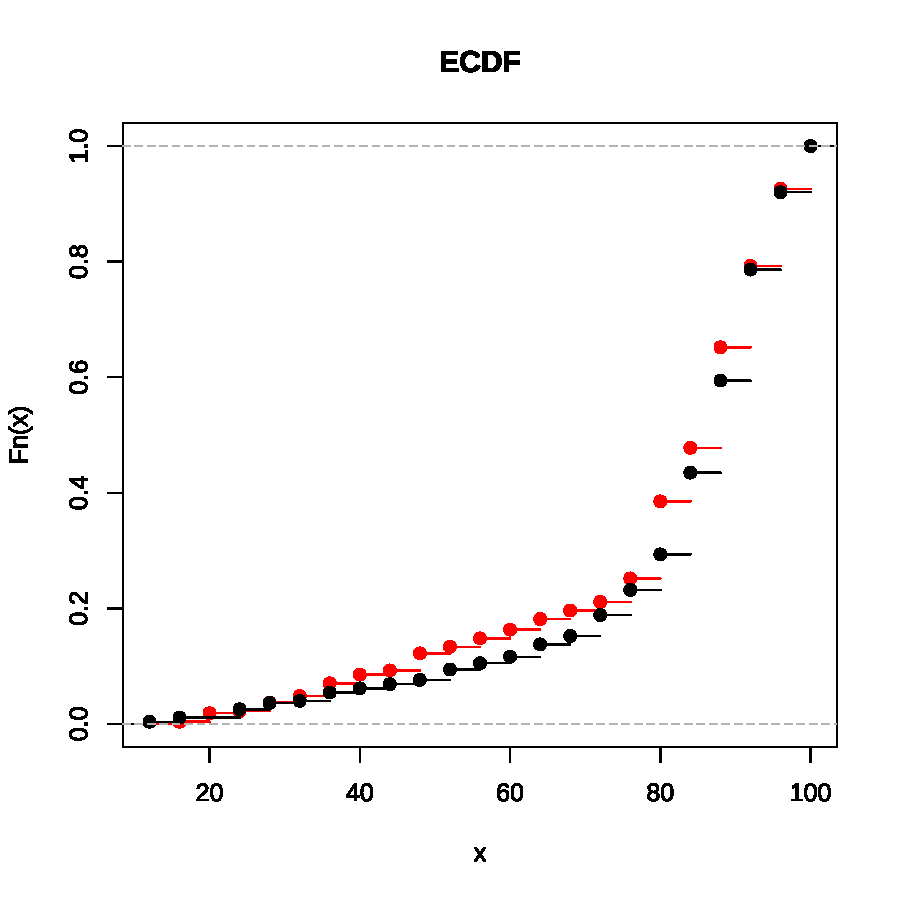
\includegraphics{Literacy_google_p_250331_v3_files/figure-latex/ECDF-1.pdf}

\subsubsection{t-test}\label{t-test}

Red 와 Black으로부터 관찰된 점수들의 평균에 대하여 t test를 적용하였더니
기초통계량에서 살핀 것을 뒷받침해 주듯이 p-value 가 0.05보다 큰 값이
나왔습니다. 평균은 닮았다는 뜻입니다.

\begin{longtable}[]{@{}
  >{\raggedleft\arraybackslash}p{(\columnwidth - 10\tabcolsep) * \real{0.1667}}
  >{\raggedleft\arraybackslash}p{(\columnwidth - 10\tabcolsep) * \real{0.0784}}
  >{\raggedleft\arraybackslash}p{(\columnwidth - 10\tabcolsep) * \real{0.0980}}
  >{\raggedleft\arraybackslash}p{(\columnwidth - 10\tabcolsep) * \real{0.2451}}
  >{\raggedleft\arraybackslash}p{(\columnwidth - 10\tabcolsep) * \real{0.1961}}
  >{\raggedleft\arraybackslash}p{(\columnwidth - 10\tabcolsep) * \real{0.2157}}@{}}
\caption{Welch Two Sample t-test: \texttt{score} by
\texttt{.\$group}}\tabularnewline
\toprule\noalign{}
\begin{minipage}[b]{\linewidth}\raggedleft
Test statistic
\end{minipage} & \begin{minipage}[b]{\linewidth}\raggedleft
df
\end{minipage} & \begin{minipage}[b]{\linewidth}\raggedleft
P value
\end{minipage} & \begin{minipage}[b]{\linewidth}\raggedleft
Alternative hypothesis
\end{minipage} & \begin{minipage}[b]{\linewidth}\raggedleft
mean in group Red
\end{minipage} & \begin{minipage}[b]{\linewidth}\raggedleft
mean in group Black
\end{minipage} \\
\midrule\noalign{}
\endfirsthead
\toprule\noalign{}
\begin{minipage}[b]{\linewidth}\raggedleft
Test statistic
\end{minipage} & \begin{minipage}[b]{\linewidth}\raggedleft
df
\end{minipage} & \begin{minipage}[b]{\linewidth}\raggedleft
P value
\end{minipage} & \begin{minipage}[b]{\linewidth}\raggedleft
Alternative hypothesis
\end{minipage} & \begin{minipage}[b]{\linewidth}\raggedleft
mean in group Red
\end{minipage} & \begin{minipage}[b]{\linewidth}\raggedleft
mean in group Black
\end{minipage} \\
\midrule\noalign{}
\endhead
\bottomrule\noalign{}
\endlastfoot
-1.433 & 538.2 & 0.1524 & two.sided & 79.93 & 82.23 \\
\end{longtable}

\subsection{문해력 등급
판정}\label{uxbb38uxd574uxb825-uxb4f1uxae09-uxd310uxc815}

\subsubsection{분포표}\label{uxbd84uxd3ecuxd45c}

\begin{itemize}
\tightlist
\item
  I수준(24점 이하), II수준(28 \textasciitilde{} 48점), III수준(52
  \textasciitilde{} 72점), IV수준(76점 이상)
\end{itemize}

\begin{longtable}[]{@{}rrrrr@{}}
\caption{문해력 등급 분포}\tabularnewline
\toprule\noalign{}
I & II & III & IV & 계 \\
\midrule\noalign{}
\endfirsthead
\toprule\noalign{}
I & II & III & IV & 계 \\
\midrule\noalign{}
\endhead
\bottomrule\noalign{}
\endlastfoot
13 & 41 & 55 & 437 & 546 \\
\end{longtable}

\begin{longtable}[]{@{}rrrrr@{}}
\caption{문해력 등급 분포(\%)}\tabularnewline
\toprule\noalign{}
I & II & III & IV & 계 \\
\midrule\noalign{}
\endfirsthead
\toprule\noalign{}
I & II & III & IV & 계 \\
\midrule\noalign{}
\endhead
\bottomrule\noalign{}
\endlastfoot
2.38 & 7.51 & 10.07 & 80.04 & 100 \\
\end{longtable}

\subsubsection{Red and Black}\label{red-and-black}

\textbf{카이제곱 테스트}로 Red와 Black에 들어간 등급별 인원수가 얼마나
닮았는지를 살펴보았지만 t-test와 마찬가지로 통계적으로 유의한 차이가
관찰되지 않았습니다.

\begin{longtable}[]{@{}lrrrrr@{}}
\caption{그룹별 문해력 등급 분포}\tabularnewline
\toprule\noalign{}
& I & II & III & IV & 계 \\
\midrule\noalign{}
\endfirsthead
\toprule\noalign{}
& I & II & III & IV & 계 \\
\midrule\noalign{}
\endhead
\bottomrule\noalign{}
\endlastfoot
Red & 6 & 27 & 24 & 213 & 270 \\
Black & 7 & 14 & 31 & 224 & 276 \\
계 & 13 & 41 & 55 & 437 & 546 \\
\end{longtable}

\begin{longtable}[]{@{}
  >{\raggedleft\arraybackslash}p{(\columnwidth - 4\tabcolsep) * \real{0.2361}}
  >{\raggedleft\arraybackslash}p{(\columnwidth - 4\tabcolsep) * \real{0.0694}}
  >{\raggedleft\arraybackslash}p{(\columnwidth - 4\tabcolsep) * \real{0.1389}}@{}}
\caption{Pearson's Chi-squared test: \texttt{.}}\tabularnewline
\toprule\noalign{}
\begin{minipage}[b]{\linewidth}\raggedleft
Test statistic
\end{minipage} & \begin{minipage}[b]{\linewidth}\raggedleft
df
\end{minipage} & \begin{minipage}[b]{\linewidth}\raggedleft
P value
\end{minipage} \\
\midrule\noalign{}
\endfirsthead
\toprule\noalign{}
\begin{minipage}[b]{\linewidth}\raggedleft
Test statistic
\end{minipage} & \begin{minipage}[b]{\linewidth}\raggedleft
df
\end{minipage} & \begin{minipage}[b]{\linewidth}\raggedleft
P value
\end{minipage} \\
\midrule\noalign{}
\endhead
\bottomrule\noalign{}
\endlastfoot
5.301 & 3 & 0.151 \\
\end{longtable}

\subsection{유형별 정답률}\label{uxc720uxd615uxbcc4-uxc815uxb2f5uxb960}

\begin{longtable}[]{@{}llr@{}}
\toprule\noalign{}
& 유형 & 정답률(\%) \\
\midrule\noalign{}
\endhead
\bottomrule\noalign{}
\endlastfoot
문1 & 사실적 & 98.4 \\
문2 & 사실적 & 93.6 \\
문3 & 비판적 & 76.9 \\
문4 & 사실적 & 95.4 \\
문5 & 추론적 & 88.3 \\
문6 & 추론적 & 68.7 \\
문7 & 추론적 & 91.9 \\
문8 & 사실적 & 79.7 \\
문9 & 추론적 & 34.1 \\
문10 & 추론적 & 88.5 \\
문11 & 사실적 & 87.9 \\
문12 & 사실적 & 66.3 \\
문13 & 사실적 & 86.8 \\
문14 & 추론적 & 87.4 \\
문15 & 사실적 & 72.3 \\
문16 & 사실적 & 81.1 \\
문17 & 추론적 & 65.0 \\
문18 & 비판적 & 90.1 \\
문19 & 사실적 & 90.7 \\
문20 & 사실적 & 80.8 \\
문21 & 사실적 & 80.6 \\
문22 & 비판적 & 73.3 \\
문23 & 추론적 & 89.2 \\
문24 & 사실적 & 79.7 \\
문25 & 추론적 & 80.8 \\
\end{longtable}

\subsection{어려운 문제?}\label{uxc5b4uxb824uxc6b4-uxbb38uxc81c}

\subsubsection{정답률 80\%
이하}\label{uxc815uxb2f5uxb960-80-uxc774uxd558}

\begin{longtable}[]{@{}lrrrrrrrrr@{}}
\toprule\noalign{}
& 문3 & 문6 & 문8 & 문9 & 문12 & 문15 & 문17 & 문22 & 문24 \\
\midrule\noalign{}
\endhead
\bottomrule\noalign{}
\endlastfoot
정답률 & 76.9 & 68.7 & 79.7 & 34.1 & 66.3 & 72.3 & 65 & 73.3 & 79.7 \\
\end{longtable}

\subsubsection{정답률 70\%
이하}\label{uxc815uxb2f5uxb960-70-uxc774uxd558}

\begin{longtable}[]{@{}lrrrr@{}}
\toprule\noalign{}
& 문6 & 문9 & 문12 & 문17 \\
\midrule\noalign{}
\endhead
\bottomrule\noalign{}
\endlastfoot
정답률 & 68.7 & 34.1 & 66.3 & 65 \\
\end{longtable}

\subsubsection{정답률 60\%
이하}\label{uxc815uxb2f5uxb960-60-uxc774uxd558}

\begin{longtable}[]{@{}lr@{}}
\toprule\noalign{}
& 문9 \\
\midrule\noalign{}
\endhead
\bottomrule\noalign{}
\endlastfoot
정답률 & 34.1 \\
\end{longtable}

\subsubsection{정답률 50\%
이하}\label{uxc815uxb2f5uxb960-50-uxc774uxd558}

\begin{longtable}[]{@{}lr@{}}
\toprule\noalign{}
& 문9 \\
\midrule\noalign{}
\endhead
\bottomrule\noalign{}
\endlastfoot
정답률 & 34.1 \\
\end{longtable}

\subsection{정답률이 낮은
문제들}\label{uxc815uxb2f5uxb960uxc774-uxb0aeuxc740-uxbb38uxc81cuxb4e4}

\subsubsection{문6.}\label{uxbb386.}

\begin{flushleft}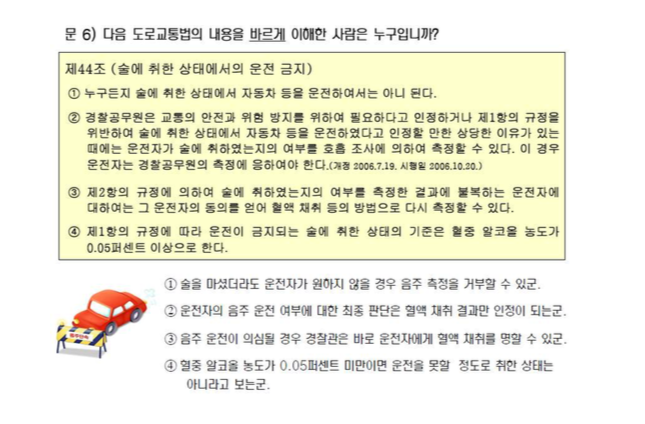
\includegraphics[width=0.75\linewidth]{./pics/Q06} \end{flushleft}

\subsubsection{문9.}\label{uxbb389.}

\begin{flushleft}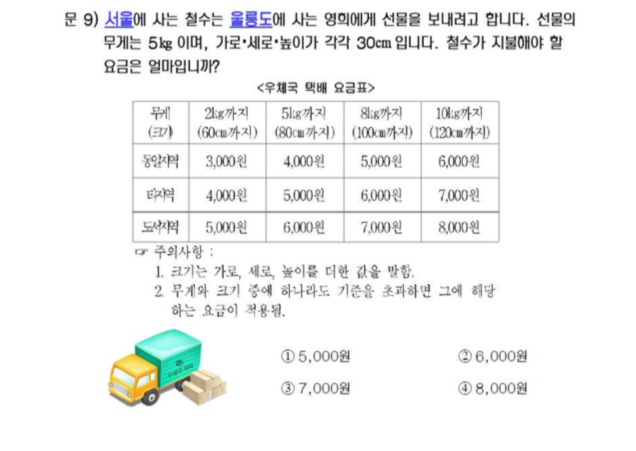
\includegraphics[width=0.75\linewidth]{./pics/Q09} \end{flushleft}

\subsubsection{문12.}\label{uxbb3812.}

\begin{flushleft}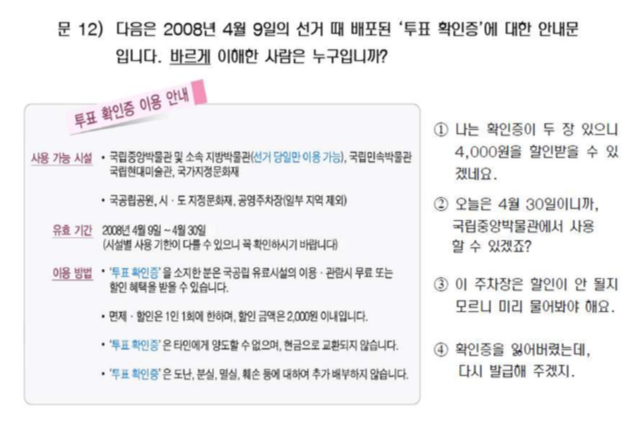
\includegraphics[width=0.75\linewidth]{./pics/Q12} \end{flushleft}

\subsubsection{문15.}\label{uxbb3815.}

\begin{flushleft}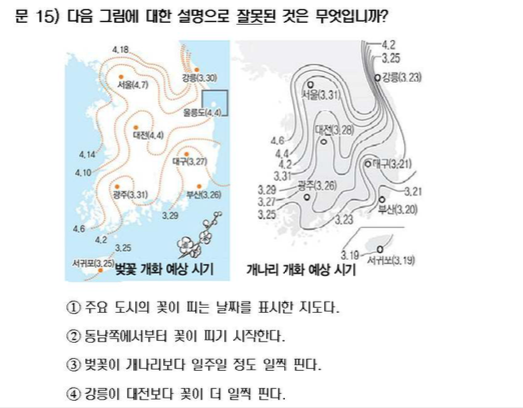
\includegraphics[width=0.75\linewidth]{./pics/Q15} \end{flushleft}

\subsubsection{문17.}\label{uxbb3817.}

\begin{flushleft}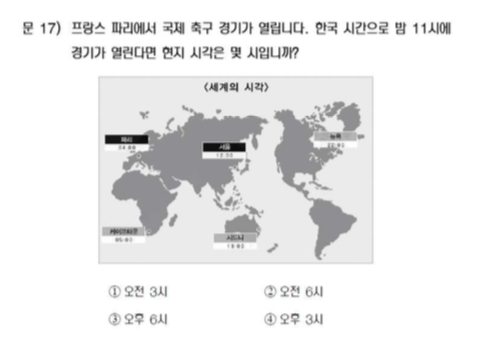
\includegraphics[width=0.75\linewidth]{./pics/Q17} \end{flushleft}

\subsubsection{문22.}\label{uxbb3822.}

\begin{flushleft}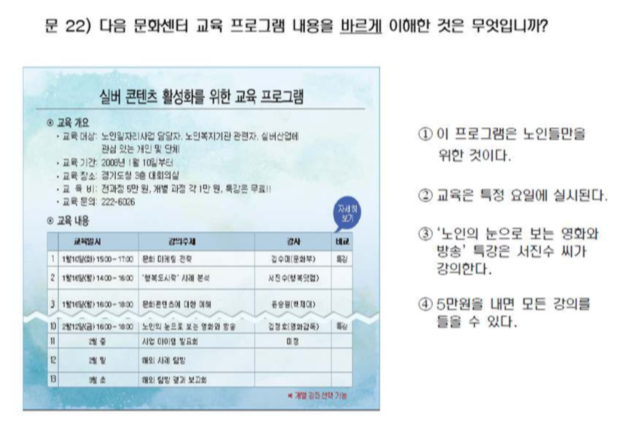
\includegraphics[width=0.75\linewidth]{./pics/Q22} \end{flushleft}

\end{document}
